\documentclass{article}
\usepackage{polski}
\usepackage[utf8]{inputenc}
\usepackage{comment}
\usepackage{enumitem}
\usepackage{graphicx}
\usepackage{hyperref}
\usepackage[section]{placeins}

\title{Baza danych FooDBall. Konstrukcja oraz użycie.}
\author{Wojciech Kulczak}
\date{Czerwiec 2019}

\begin{document}

\maketitle
\newpage
\section{Wprowadzenie}
\begin{comment}
Stuff z wprowadzenia, później już zasady
\end{comment}
Baza ta przedstawia dane dotyczące rozgrywek ligii piłki nożnej. \newline
W konstukcji tej bazy postawiono wspólne wymagania:
\begin{enumerate}
    \item Zawodnicy przypisani są do drużyn
    \item \label{zmiana} W jednym sezonie przypisanie jest stałe a w wielu sezonach może być różne
    \item Drużyny rozgrywają w sezonie 2 mecze każdy z każdym: w każdym meczu biorą udział dwie drużyny- jedna pełni rolę gospodarza, druga gościa
    \item Rejestrowane są dane o przebiegu meczu: kto grał i w jakim czasie, kto i kiedy strzelił bramkę, kto i kiedy otrzymał kartkę 
\end{enumerate}
Dodano również kilka dodatkowych zasad:
\begin{enumerate}[resume]
    \item Rejestrowane są dane o zmianach podczas meczu, podczas jednego meczu jedna strona nie może dokonać więcej niż trzech zmian.
    \item Zapisane są informacje o frekwencji widowni podczas meczu 
    \item Każda z drużyn posiada swojego kapitana i trenera, którzy zmieniać się mogą na zasadzie opisanej w podpunkcie \ref{zmiana}. 
\end{enumerate}
\newpage
\section{Opracowanie diagramu ER}
\begin{figure}[!h]
    \centering
    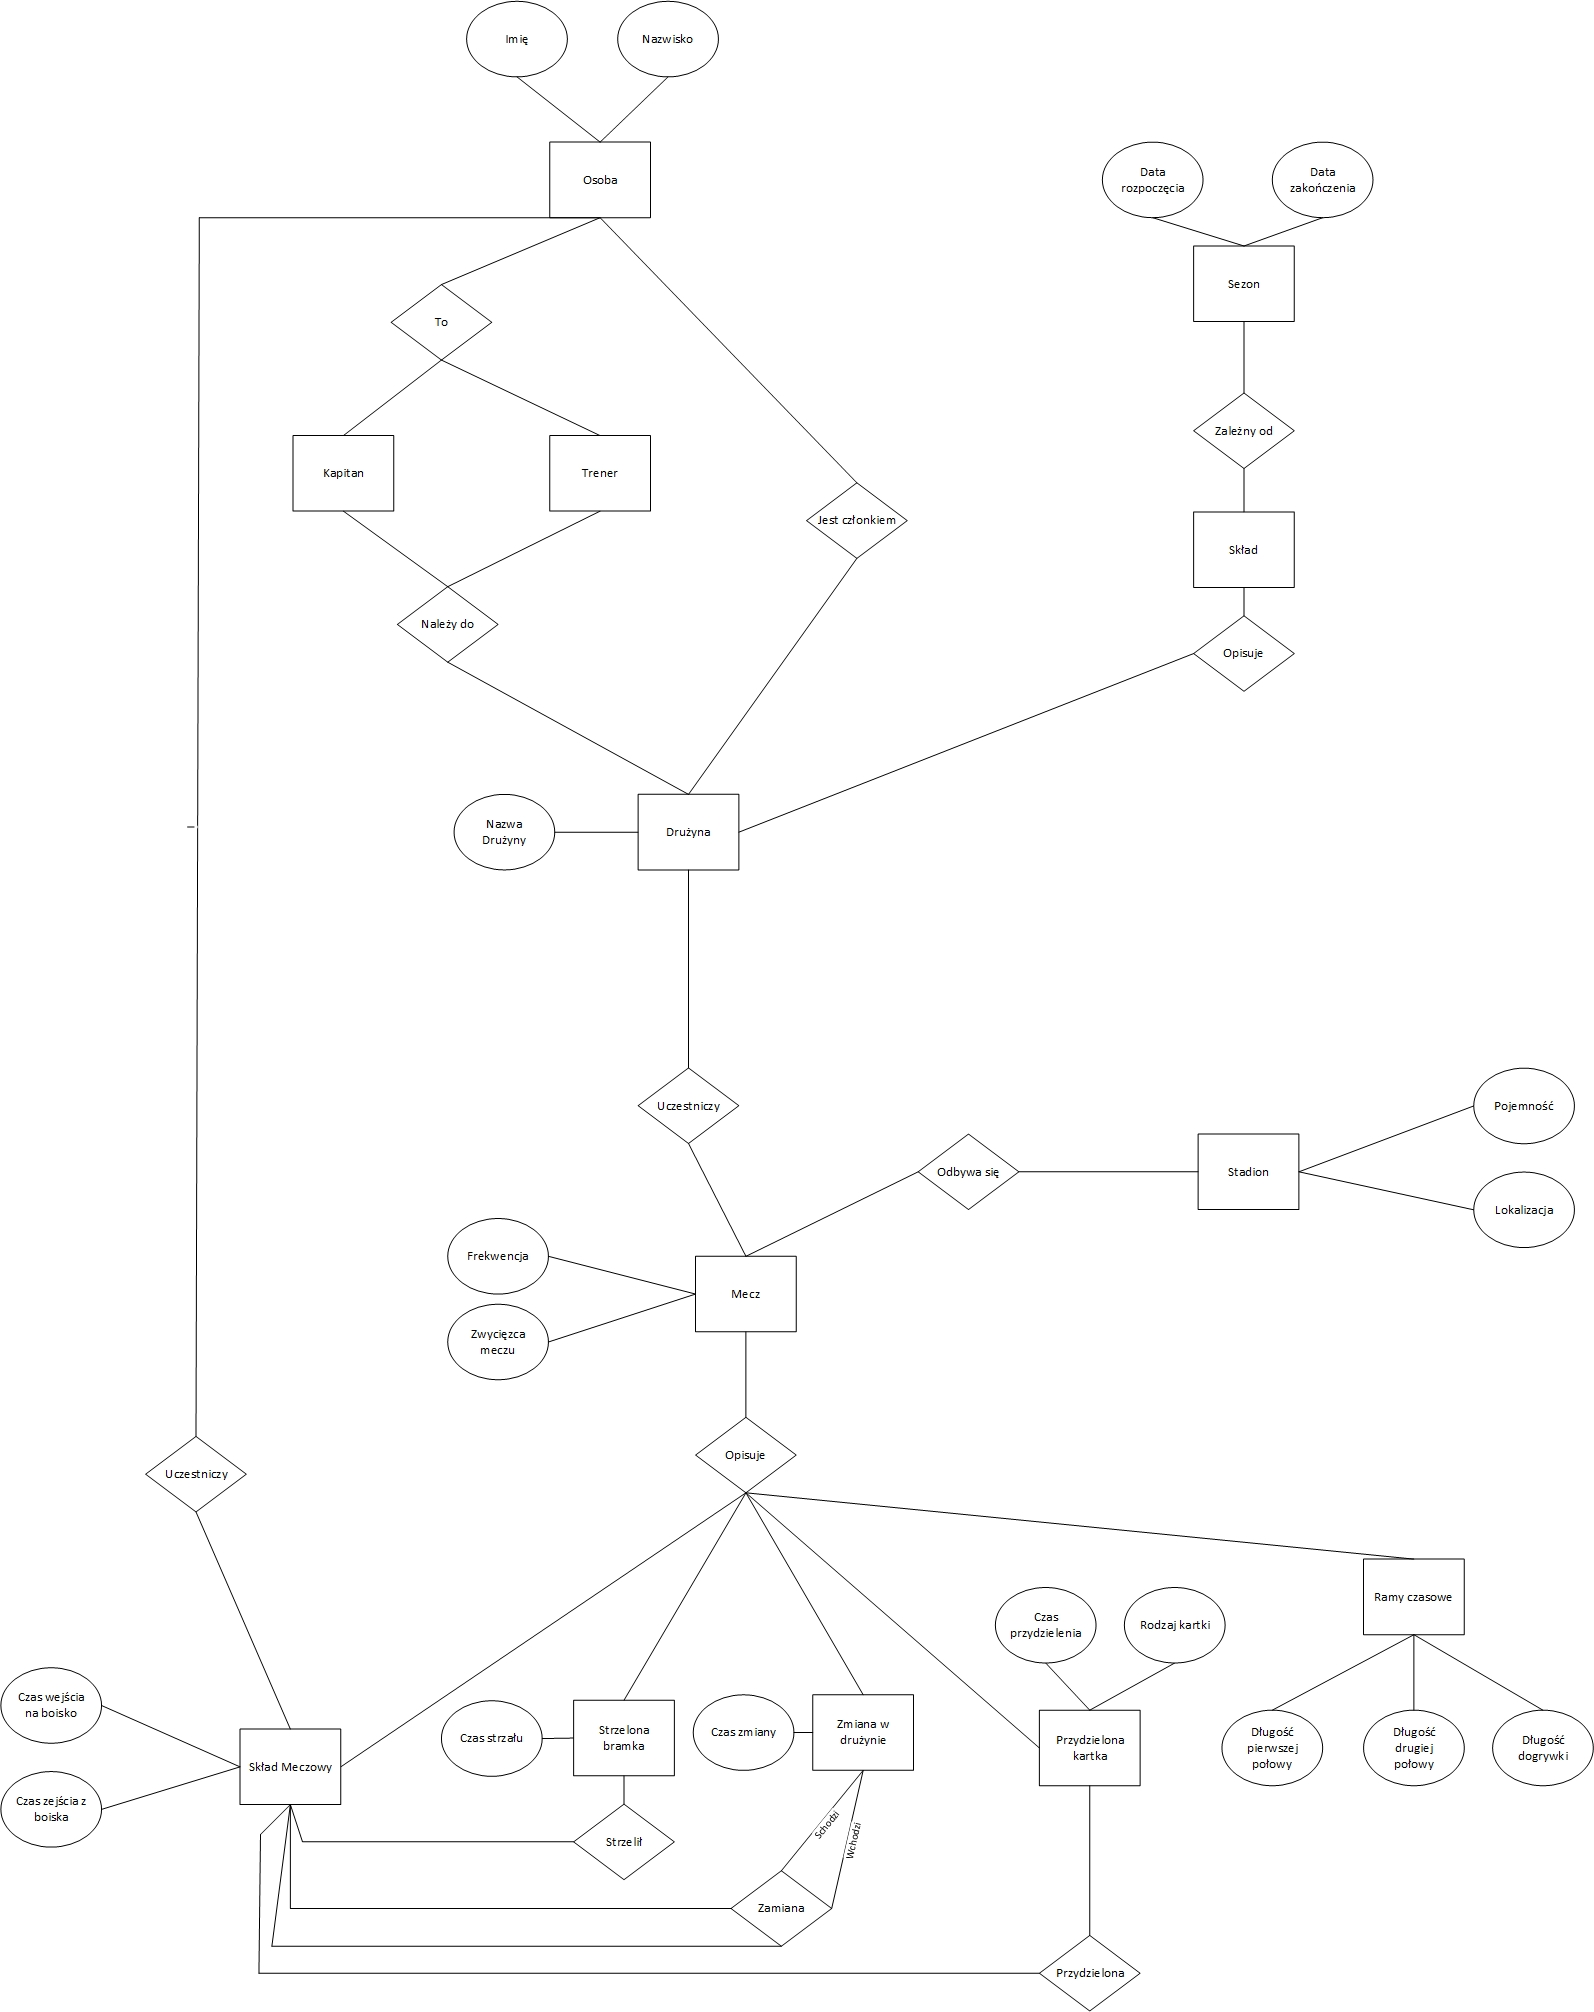
\includegraphics[width=\textwidth,keepaspectratio]{ER.jpg}
    \caption{Diagram ER}
    \label{ER}
\end{figure}
\newpage
\section{Generacja diagramu ERD}
\begin{figure}[!h]
    \centering
    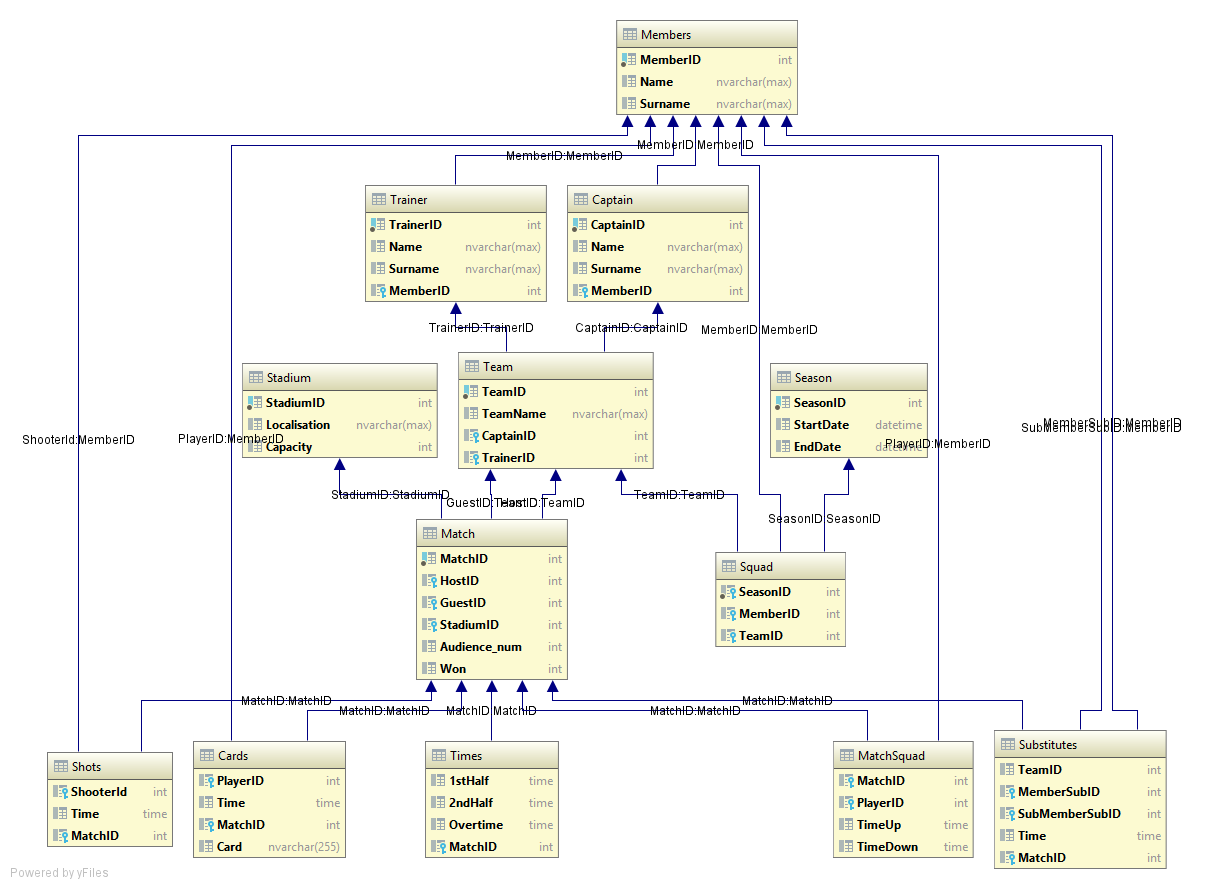
\includegraphics[width=10cm,keepaspectratio]{dbo_DG.png}
    \caption{Diagram ERD wygenerowany przez DataGrip}
    \label{ERD_Datagrip}
\end{figure}
\section{Definicja bazy danych w SQL}
Poniżej umieszczono skrypty generacji każedej z tablic wraz z relacjami
\begin{verbatim}

    CREATE TABLE members 
  ( 
     memberid INT NOT NULL CONSTRAINT members_pk UNIQUE, 
     NAME     NVARCHAR(max), 
     surname  NVARCHAR(max) 
  ) 
go 
\end{verbatim}
\newpage
\begin{verbatim}
CREATE TABLE captain 
  ( 
     captainid INT NOT NULL CONSTRAINT captain_pk UNIQUE, 
     NAME      NVARCHAR(max), 
     surname   NVARCHAR(max), 
     memberid  INT CONSTRAINT captain_members_memberid_fk REFERENCES members ( 
     memberid 
     ) 
  ) 
go 
CREATE TABLE season 
  ( 
     seasonid  INT NOT NULL CONSTRAINT season_pk UNIQUE, 
     startdate TIME, 
     enddate   TIME 
  ) 
go 
CREATE TABLE stadium 
  ( 
     stadiumid    INT NOT NULL CONSTRAINT stadium_pk UNIQUE, 
     localistaion NVARCHAR(max), 
     capacity     INT 
  ) 
go 
CREATE TABLE trainer 
  ( 
     trainerid INT NOT NULL CONSTRAINT trainer_pk UNIQUE, 
     NAME      NVARCHAR(max), 
     surname   NVARCHAR(max), 
     memberid  INT CONSTRAINT trainer_members_memberid_fk REFERENCES members ( 
     memberid 
     ) 
  ) 
go 
CREATE TABLE team 
  ( 
     teamid    INT NOT NULL CONSTRAINT team_pk UNIQUE, 
     teamname  NVARCHAR(max), 
     captainid INT CONSTRAINT team_captain_captainid_fk REFERENCES captain ( 
     captainid 
     ), 
     trainerid INT CONSTRAINT team_trainer_trainerid_fk REFERENCES trainer ( 
     trainerid 
     ) 
  ) 
go 
CREATE TABLE match 
  ( 
     matchid      INT NOT NULL CONSTRAINT match_pk UNIQUE, 
     hostid       INT CONSTRAINT match_team_teamid_fk_2 REFERENCES team (teamid) 
     , 
     guestid      INT CONSTRAINT match_team_teamid_fk REFERENCES team ( 
     teamid), 
     stadiumid    INT CONSTRAINT match_stadium_stadiumid_fk REFERENCES stadium ( 
     stadiumid), 
     audience_num INT, 
     won          INT 
  ) 
go 
CREATE TABLE cards 
  ( 
     playerid INT CONSTRAINT cards_members_memberid_fk REFERENCES members ( 
     memberid), 
     time     TIME, 
     matchid  INT CONSTRAINT cards_match__fk REFERENCES match (matchid), 
     card     NVARCHAR(255) 
  ) 
go 
CREATE TABLE matchsquad 
  ( 
     matchid  INT CONSTRAINT matchsquad_match__fk REFERENCES match (matchid), 
     playerid INT CONSTRAINT matchsquad_members_memberid_fk REFERENCES members ( 
     memberid), 
     timeup   TIME, 
     timedown TIME 
  ) 
go 
CREATE TABLE shots 
  ( 
     shooterid INT CONSTRAINT shots_members_memberid_fk REFERENCES members ( 
     memberid), 
     time      TIME, 
     matchid   INT CONSTRAINT shots_match__fk REFERENCES match (matchid) 
  ) 
go 
\end{verbatim}
\newpage
\begin{verbatim}
CREATE TABLE squad 
  ( 
     seasonid INT NOT NULL CONSTRAINT squad_season_seasonid_fk REFERENCES season 
     ( 
     seasonid), 
     memberid INT CONSTRAINT squad_members_memberid_fk REFERENCES members ( 
     memberid), 
     teamid   INT CONSTRAINT squad_team_teamid_fk REFERENCES team (teamid) 
  ) 
go 
CREATE TABLE substitutes 
  ( 
     teamid         INT, 
     membersubid    INT CONSTRAINT substitutes_members_memberid_fk_2 REFERENCES 
     members 
     (memberid), 
     submembersubid INT CONSTRAINT substitutes_members_memberid_fk REFERENCES 
     members 
     (memberid), 
     time           TIME, 
     matchid        INT CONSTRAINT substitutes_match__fk REFERENCES match ( 
     matchid) 
  ) 
go 
CREATE TABLE times 
  ( 
     [1sthalf] TIME, 
     [2ndhalf] TIME, 
     overtime  TIME, 
     matchid   INT CONSTRAINT times_match__fk REFERENCES match (matchid) 
  ) 
go 
\end{verbatim}
Folder skryptów genereracji bazy danych znaleźć można na stronie: \url{github.com}
\newpage
\section{Zastosowanie bazy. Przykładowe zapytania języka SQL}
Zaprojektowaną bazę danych planuję rozszerzyć o interfejs graficzny w formie aplikacji lub strony internetowej, tak, by przypominało format danych zawarty na stronie \url{pzpn.pl}.
Baza została zaprojektowana w taki sposób, by z połączenia odpowiednio małych tabel uzyskać wszystkie informacje, którymi jesteśmy zainteresowani.
\newline
Przykład: Wyświetl członków poszczególnych drużyn w pierwszym sezonie:
\begin{verbatim}
    SELECT [TeamName],[Name], [Surname] from Members
    INNER JOIN Squad on Squad.MemberID=Members.MemberID
    INNER JOIN Team on Team.TeamID=Squad.TeamID
    WHERE SeasonID=0
\end{verbatim}

\begin{comment}
Do wykonania projektu użyłem oprogramowania:
\begin{list}
    \item Jetbrains DataGrip
    \item Microsoft Access
    \item Microsoft SQL Server Management Studio
\end{list}
\end{comment}



\end{document}
